\documentclass[12pt]{article}
\usepackage{graphicx}
\begin{document}
\title{jArk \\\small A Java arkanoid implementation \\ User Guide }
\author{Pongelli Stefano \and Thomas Selber} 
\date{\today}
\maketitle
\newpage
\tableofcontents
\newpage
\section{The game}
\label{sec:go}

\subsection{Introduction}
\label{sec:intro}

Arkanoid is a classical Arcade game, the player controls a paddle called Vaus which moves horizontally. This paddle has to prevent a ball from falling out of the screen, bouncing it thowards the brick field on the top.\\
When the ball hits a brick the brick get destroyed (or loses a life in case of multi-hit brick). Sometimes the brick contains a bonus, which will be dropped thowards the Vaus as soon as the brick is destroyed.\\
To win the game the player has to destroy all the bricks (except for those which cannot be destroyed).

\newpage
\section{jArk}

\subsection{How to play}
This game is made in Java, therefore to play it you'll need a Java Virual Machine.\\\\
The main file is called ``jArk.jar'', you just have to double click it and the game will start.\\\\
A ``levels/'' directory and a ``HighScore'' file will be automatically created.\\

\subsection{Commands}
\label{sec:intro}

You can either move the Vaus with the keyboard (left and right arrows), or with the mouse. \\
Press Esc to pause or resume teh game.\\
Press Space to shoot (either with the rifles or the cannon), and click with the mouse to release the balls (i.e. Stick ball, or Starting ball).\\
\\
Either way, you will need to use the Mouse, so we advise you to play with it.\\

\newpage
\subsection{Main window}

\begin{figure}[htbp]
  \centering
    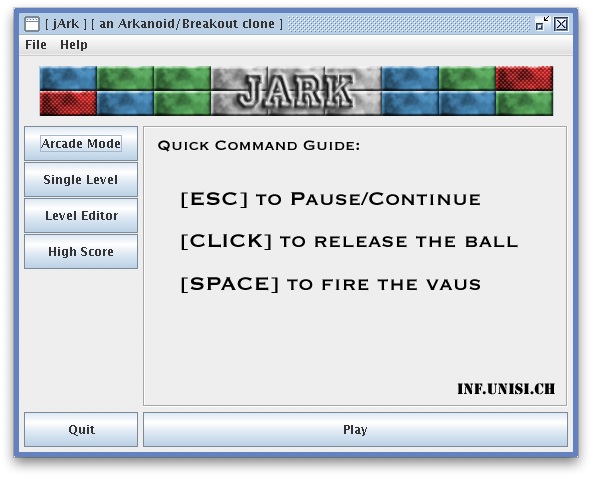
\includegraphics[scale=0.6]{mainscreen.png}
  \caption{Main Window (GUI)}
  \label{guimain}
\end{figure}
This is the main game window, from this window one can start a new Arcade game, select a single level, create a level with the level editor or see the current high score.\\
\newpage

\subsubsection*{1. Arcade Mode}
This is the classic modality, the player goes through all the default levels and at the end (or when a gemeover occours) he can save his score.\\
\subsubsection*{2. Single Level}
This section lets the user choose to play a level.\\
The levels are taken from the user created levels (in the ``levels/'' folder) and also from the already finished levels. In other words each time the player clears a level in arcade mode, the levels get copied into the ``levels/'' folder thus beeing accessible to be played or modified.\\
\begin{figure}[htbp]
  \centering
    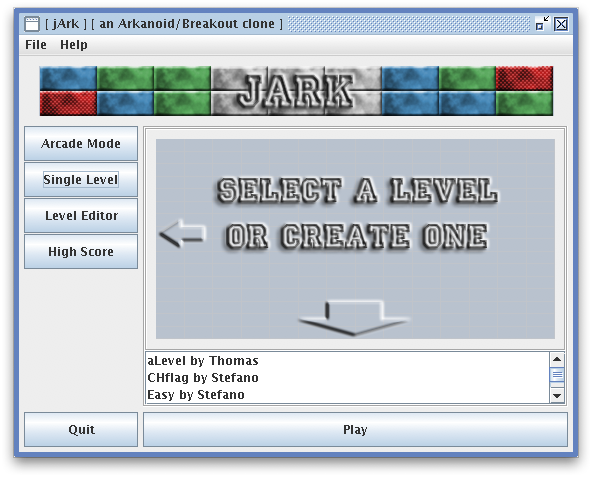
\includegraphics[scale=0.6]{singlelevel.png}
  \caption{Single level (GUI)}
  \label{guimain}
\end{figure}

\subsubsection*{3. Level editor}
This button will open a new level editor.\\
Levels can be created, loaded, and stored.\\
More information below.

\subsubsection*{6. High Score}
This displays the High Score of the Arcade Mode.\\

\newpage
\subsection{Game window}
 
\begin{figure}[htbp]
  \centering
    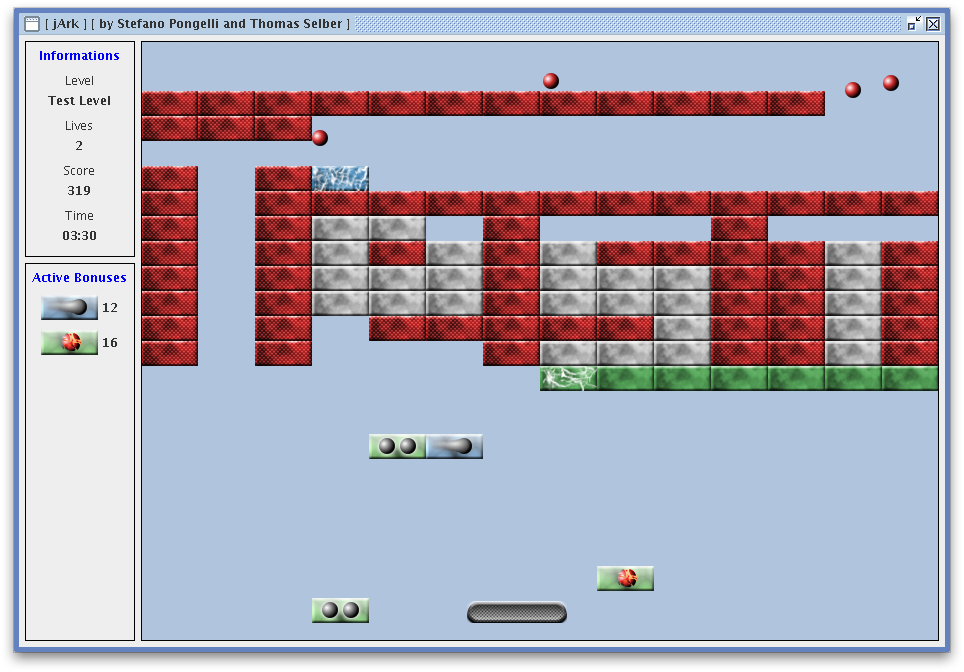
\includegraphics[scale=0.4]{gamewindow.png}
  \caption{Game window (GUI)}
  \label{guigame}
\end{figure}
This is the game window, you can see on the lefthand side two panels: information and active bonuses, with self explaining names (the number on the right of the active bonuses is the time remaining for that bonus effect).\\
In the middle the is the main game screen with the Vaus, some bonuses falling down, and some different kind of bricks.\\
This will be explained below.\\
\newpage
\subsubsection*{1. Bricks}
There are four types of bricks: \\
the default is destroyed with 1 hit;\\
the resistent with 2 hits; and \\
the very resistent with 3 hits.\\
The persistent cannot be destroyed (doesn't count as a brick at the end).\\
\begin{figure}[htbp]
  \centering
    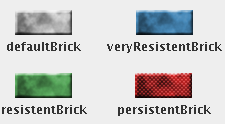
\includegraphics[scale=0.7]{bricks.png}
  \caption{Bricks}
  \label{buddies}
\end{figure}

\subsubsection*{2. Vaus}
There are five types of Vaus:\\
the default, with a rifle, with 2 rifles and with a cannon;\\
plus the long one and the short one.\\
There can also be a long rifle vaus, or short cannon vaus, and so on.\\

\begin{figure}[htbp]
  \centering
    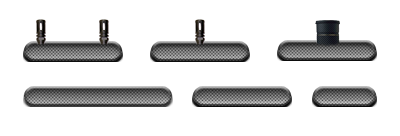
\includegraphics[scale=0.7]{vauses.png}
  \caption{Vauses}
  \label{buddies}
\end{figure}

\subsubsection*{3. Bonus}
We have 18 different bonuses, the names are self explaining and you can see a quich guide pressing ESC during a game (pause).\\
\begin{figure}[htbp]
  \centering
    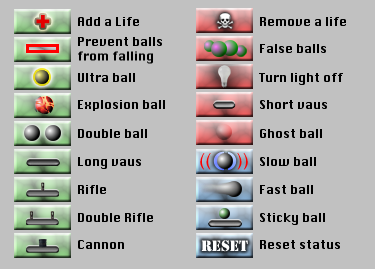
\includegraphics[scale=0.7]{bonuses.png}
  \caption{Bonuses}
  \label{buddies}
\end{figure}

\subsubsection*{4. Balls}
We also have different types of balls: default, explosion, ultra, false, ghost, and sticky.
\begin{figure}[htbp]
  \centering
    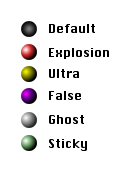
\includegraphics[scale=0.7]{balls.png}
  \caption{Balls}
  \label{buddies}
\end{figure}

\newpage
\subsection{Level Editor}
\begin{figure}[htbp]
  \centering
    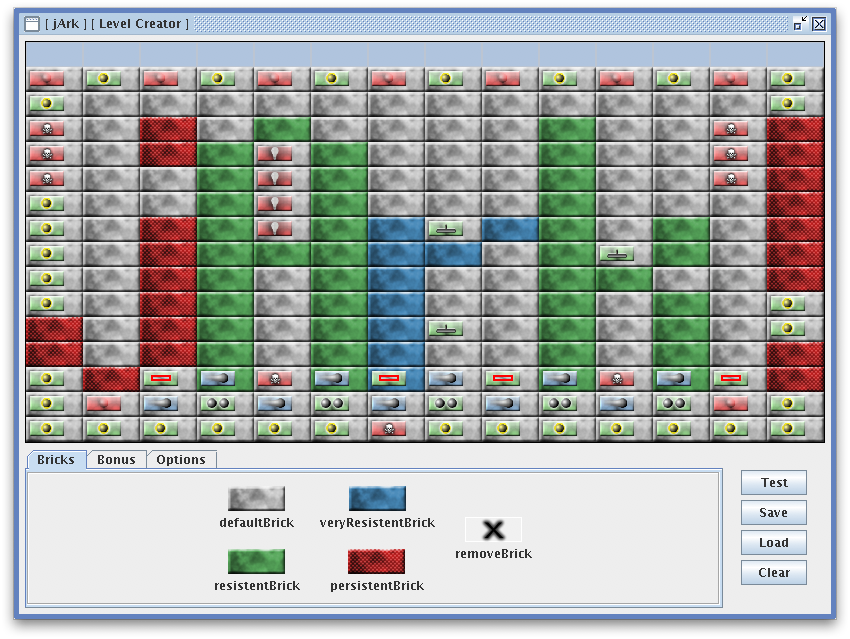
\includegraphics[scale=0.5]{editor.png}
  \caption{Level Editor}
  \label{buddies}
\end{figure}

As you can see from this image, the editor only show the bricks area: the player can create a level specifying the type and the location of each brick, and of each bonus.\\
Bonuses are shown as small icons inside the bricks, and to remove them it's just necessary to replace the brick with another one, or remove it with the brick eraser tool.\\

\subsubsection*{1. Panels}
There are three panels in this frame: the brick (shown in the picture above), the bonus and the option panel.\\

\begin{figure}[htbp]
  \centering
    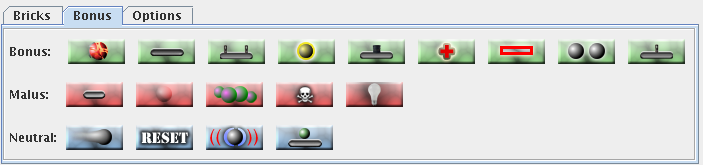
\includegraphics[scale=0.5]{bonus.png}
  \caption{Bonus Panel}
  \label{buddies}
\end{figure}

\begin{figure}[htbp]
  \centering
    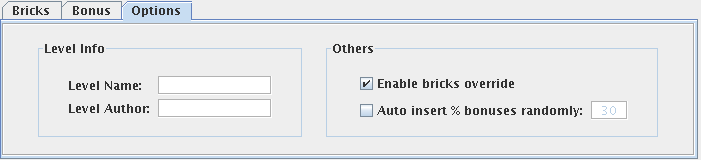
\includegraphics[scale=0.5]{options.png}
  \caption{Option Panel}
  \label{buddies}
\end{figure}

You can choose to insert bonuses from the bonus panel, or enable the ``Auto insert \% bonuses randomly" option, specifying a percentage (default 30\%). Enabling this option each time the level starts that percentage of bonuses will be randomly added.\\
Deselecting ``Bricks ovverride'' you will not be able to put bricks over other bricks already on the screen.\\
Name and Author have to be specified for each level.

\subsubsection*{2. Buttons}
You can either Test the level you are creating (a new instance of the game will start, nothing will be created), Save the current level in a file (you will have to specify the File name - which can be different from the level name), Load a previously created level or an Arcade level which has already been cleared, or Clear the current level (all bricks will be removed).
 
\newpage
\section{Credits}
\label{sec:credits}
This game has been made in a month, during the course ``Programming Fundamentals 2 (Java)'', at USI (Faculty of Informatics), Lugano, Switzerland.\\

Created by:
\begin{itemize}
\item Stefano Pongelli (stefano.pongelli@lu.unisi.ch)
\item Thomas Selber (thomas.selber@lu.unisi.ch)
\end{itemize}

~\\

Thanks to:
\begin{itemize}
\item Prof. Matthias Hauswirth
\item Andrea Adamoli
\item Krzysztof Zawadzki
\end{itemize}
\end{document}